
 
\documentclass[11pt]{article}
\addtolength{\oddsidemargin}{-1.cm}
\addtolength{\textwidth}{2cm}
\addtolength{\topmargin}{-2cm}
\addtolength{\textheight}{3.5cm}
\newcommand\tab[1][1cm]{\hspace*{#1}}
\usepackage[pdftex]{graphicx}
\usepackage{pdflscape}
\usepackage{hyperref}
\usepackage[T1]{fontenc}
\usepackage{float}
\usepackage{cite}
\hypersetup{
	colorlinks=true,
	linkcolor=black,
	filecolor=magenta,
	urlcolor=cyan,
}

% define the title
\author{Panda Inc}
\title{Catura - Purchase Management System}
\begin{document}
\begin{titlepage}
	
	\begin{center}
		% Upper part of the page         
        
\includegraphics[width=0.7\linewidth]{Images/PandaInc_logo.jpg}\\[1cm] 
		\textsc{\LARGE Panda Inc}\\[0.3cm]
		% Title
		\rule{\linewidth}{0.5mm} \\[1cm]
		{ \huge \bfseries Catura - Purchase Management System}\\[0.5cm]
		\rule{\linewidth}{0.5mm} \\[1cm] 		
  
		
		\begin{minipage}{0.4\textwidth}
			\begin{flushleft} \large
				\emph{} \\
				Quinton {Swanepoel}
			\end{flushleft}
		\end{minipage}
		\begin{minipage}{0.4\textwidth}
			\begin{flushright} \large
				\emph{} \\
				15245510
			\end{flushright}
		\end{minipage}

		\begin{minipage}{0.4\textwidth}
			\begin{flushleft} \large
            	\emph{} \\
				Azhar {Patel}
			\end{flushleft}
		\end{minipage}
		\begin{minipage}{0.4\textwidth}
			\begin{flushright} \large
				\emph{} \\
				15052592
			\end{flushright}
		\end{minipage}
		
		\begin{minipage}{0.4\textwidth}
			\begin{flushleft} \large
				\emph{} \\
				Tshepo Macebo {Malesela}
			\end{flushleft}
		\end{minipage}
		\begin{minipage}{0.4\textwidth}
			\begin{flushright} \large
				\emph{} \\
				14211582
			\end{flushright}
		\end{minipage}

		\begin{minipage}{0.4\textwidth}
			\begin{flushleft} \large
				\emph{} \\
				Monkeli Fred {Dilapisho}
			\end{flushleft}
		\end{minipage}
		\begin{minipage}{0.4\textwidth}
			\begin{flushright} \large
				\emph{} \\
				15074260
			\end{flushright}
		\end{minipage}
        
        \begin{minipage}{0.4\textwidth}
			\begin{flushleft} \large
				\emph{} \\
				Keaton {Pennels}
			\end{flushleft}
		\end{minipage}
		\begin{minipage}{0.4\textwidth}
			\begin{flushright} \large
				\emph{} \\
				14373018
			\end{flushright}
		\end{minipage}
		
		\rule{\linewidth}{0.5mm} \\[1cm] 
		\textsc{\Large Stakeholders}\\[1cm]	
		
		\begin{minipage}{0.4\textwidth}
			\begin{flushleft} \large
				\emph{} \\
				Catura:
			\end{flushleft}
		\end{minipage}
		\begin{minipage}{0.4\textwidth}
			\begin{flushright} \large
				\emph{} \\
				Diederik Mostert
			\end{flushright}
		\end{minipage}

		
	\end{center}
\end{titlepage}

\newpage
\tableofcontents
\newpage

\section{Panda Inc.}
\subsection{About Us}
Panda Inc. is a team of hard working passionate software developers. Each member of the team brings their own unique, diverse skill set to the table, which includes competence in a wide range of fields such as Artificial Intelligence, multimedia and also business intellect. Panda Inc. has a fun and modern culture that promotes blue sky thinking and solutions that fit into the modern environment. The team works exceptionally well together and all members aim to produce a quality product while also creating a constructive relationship with our client.

\subsection{The Team}
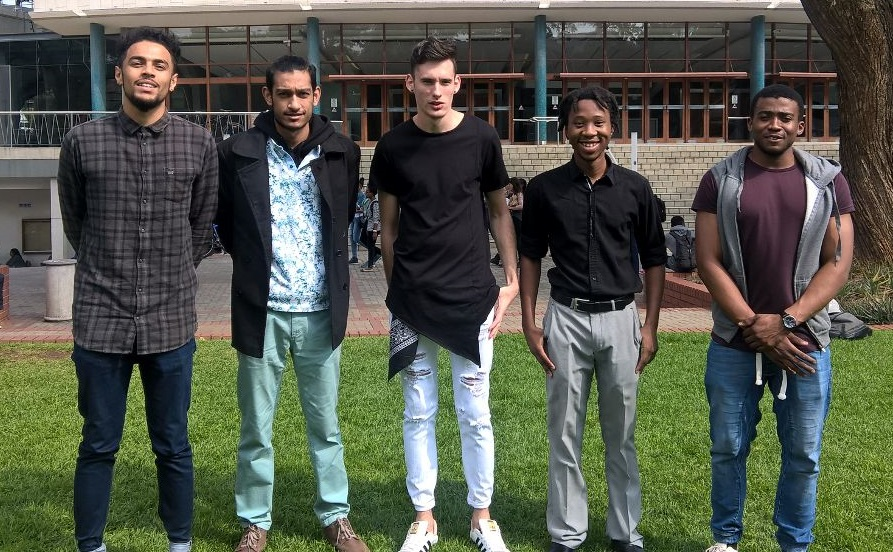
\includegraphics[width=\textwidth]{Images/Team_Pic.jpg}

\subsubsection{Quinton Swanepoel} 
\paragraph{}Course : BSc Computer Science (with Infomratics)
\paragraph{}Career Interest : Software Development / Business Systems Development  
\paragraph{}Skills : 
\begin{itemize}
\item Programming (C++, Java, C\#)
\item Web Development
\item Systems Design
\item Mobile Development (Android Studio, Xamarin)
\end{itemize}
\paragraph{Bio :}I started at the University of Pretoria in 2015 studying computer science, second year I  decided to start taking the prescribed BCom Informatics modules in addition to my computer science modules. This is because I love the business aspect of IT but I'm also interested in the deeper back-end development sector and wish to have as much knowledge as I can about systems development, front-end development, and back-end development which is not all taught in one degree. I am passionate about what I am studying which makes putting in the extra effort to always produce a perfect product that much easier. 

\subsubsection{Azhar Patel}
\paragraph{}Course : BSc Computer Science
\paragraph{}Career Interest : Software/Game Development and Security
\paragraph{}Skills : 
\begin{itemize}
\item Adept in C++ and Java
\item HTML with PHP and JavaScript
\item Mobile Development in Android
\item Artificial Intelligence 
\end{itemize}
\paragraph{Bio :}Currently in my final year at the University of Pretoria having started in 2015. I've enjoyed Psychology as an elective in my first year and it has enhanced my enthusiasm for Psychology in the Computer Science field, hence choosing a Multimedia module that focuses on Human-Computer Interaction along with gaming. Prior to University, I had a great interest in computers and excelled in Mathematics. Computer Science is composed of all of the aforementioned aspects and my passion for the field has grown eversince. I like meeting new people and solving a variety of different problems. I also enjoy online gaming which keeps my mind alert. I am dilligent and will sacrifice sleep if needed. Furthermore, I am a loyal guy and this will be portrayed one day towards the company that employs me. My final goal is to one day help people in need, possibly via programming and applications. We cannot help everyone in the world, but helping a few people can go a long way in helping many in need.

\subsubsection{Tshepo Macebo Malesela}
\paragraph{}Course : BSc Computer Science
\paragraph{}Career Interest : Software Engineering and Component Development
\paragraph{}Skills : 
\begin{itemize}
\item Programmed in C++ and java, the focus was mainly Object-oriented languages.
\item C, mainly at work, with .Net Core, MVC 6 and domain development.
\item HTML, component develepment with polymer and angular.
\item Javascript, for functionality on front-end development.
\item PHP, during my first and second year
\end{itemize}
\paragraph{Bio :} I am a student studying computer science at the University of Pretoria with a strong passion for system development and component development. Before University I believed I was going to study mathematics because at the time I really enjoyed it but by the time I had began my matric year I realised that I had a strong passion for computers, and systems. I am comfortable with front-end and back-end development. Being a student and a part-time worker has given me the skill of learning very quickly. I am very friendly, I would describe myself as a peoples person. Communication is very important to me, I honestly believe good communication makes working easier because everyone know where everyone stands. I am beginning to learn and love the business side of software development (i.e the software engineering), because I have learned that in order to make a good software product there is much more than just the good software development that is required to make the application a product. I am still learning and developing my skill as a programmer and I enjoy challanges.

\subsubsection{Monkeli Fred Dilapisho}
\paragraph{}Course : BSc Computer Science
\paragraph{}Career Interest : Software Development
\paragraph{}Skills : 
\begin{itemize}
\item Multimedia - Website Development
\item Proficient in Java and C++ Object Oriented Programming.
\item Artificial Intelligence
\end{itemize}
\paragraph{Bio :}  Having started this degree in 2015, I am a final year student at the University of Pretoria. My interest in computer science is born from IT classes in high school as well as my innate propensity for desconstructing computer technologies if only to understand better how they work. I have a long history of being dedicated to long term projects and my commitment to choral activities at the University of Pretoria is proof of this. I have an unwavering interest in developing artificial intelligence based off of maps of the human brain and find the question of mapping every connection in the human brain to be an interesting and challenging one.

\subsubsection{Keaton Pennels}
\paragraph{}Course : BSc Computer Science 
\paragraph{}Career Interest : Software Engineering, Social Entrepreneurship
\paragraph{}Skills :
\begin{itemize}
\item Programming in Object Oriented Languages such as Java, C++, C
\item Competent in Assembly (Intel)
\item Web Development - Experienced in both the LAMP(Linux, Apache, MySQL, PHP) stack and the MEAN (MongoDB, Eclipse, AngularJS, Node) stack as well as MVC based implementation.
\item Project Management
\end{itemize}
\paragraph{Bio :}I am a second generation Software Engineer, inspired by my mother to pursue a career in Computer Science. I see software engineering as a means to not only engage myself in the technologically driven world we live in, but also as a conduit to producing products and services for the empowerment of the general masses. Software Engineering is a field of work that I am highly passionate about and it is my intention to commit the rest of my life to perfecting skills required to be a stand out operative, with respect to both the programming and engineering aspects of the field.

\section{Motivation For Project}
When looking for a project that allowed for an implementation of many different fields of study within the computer science field, Catura's Cloud based purchase management system. caught our groups attention. It allows for the integration of computer science and e-commerce to create a product that will both make purchases easier for users and the suppliers. 
\newline When choosing this project, the team assessed each of our skills thoroughly and given that we have on our team members who are currently enrolled in an Artificial Intelligence course, members who have been exposed to the business aspect of IT and some of our members have experience developing in domain of this project and have had exposure to the processes required for creating , we believed this project was well suited for our group
\newline In addition to our joint knowledge in these fields, we  also have experience in research and information handling and as such, as a group we are also very comfortable with learning new technologies to optimize the system as best as possible.As a group we know that this project plays to the teams strength while also allowing us to be innovative and challenged.
\section{The Project}
\subsection{High Level Description}
The system is a purchase management system which must allow users the ability to search for products offered by different wholesalers. The system should allow the user to compare product prices from the various wholesalers. The details of each product should be very clear and describe the product very well, the product information should be provided by the wholesalers. When a user searches for a product, they will use a keyword a phrase associated with the product and if the product exists within the system, it should be listed with the same or similar product from other wholesalers.
\begin{itemize}
\item There are two main types of account holders, wholesalers or suppliers and consumers.
\item All account holders have to register with the system and the system will have a verification method to check user data.
\item Account holders looking to purchase a product need to search for the product, make an order which should include the the number of items the account holder wants, and the system must provide a payment method.
\item The system must provide a method for suppliers to do CRUD operations on the stock available.
\end{itemize}

\subsection{Technologies To Be Used}
\subsubsection{Front-End}
\begin{itemize}
\item (Web-Interface) HTML5, CSS3, Javascript, Polymer.
\item (Mobile-Interface) Android Studio (java), 
\end{itemize}
\subsubsection{Back-End}
\begin{itemize}
\item Java for the server development.
\item Object-Oriented Database such as db4o will be used to store data.
\item Cloud-based servers to provide the hosting such as Amazon web services.
\end{itemize}
\subsection{Deployment Diagram}
\begin{center}
 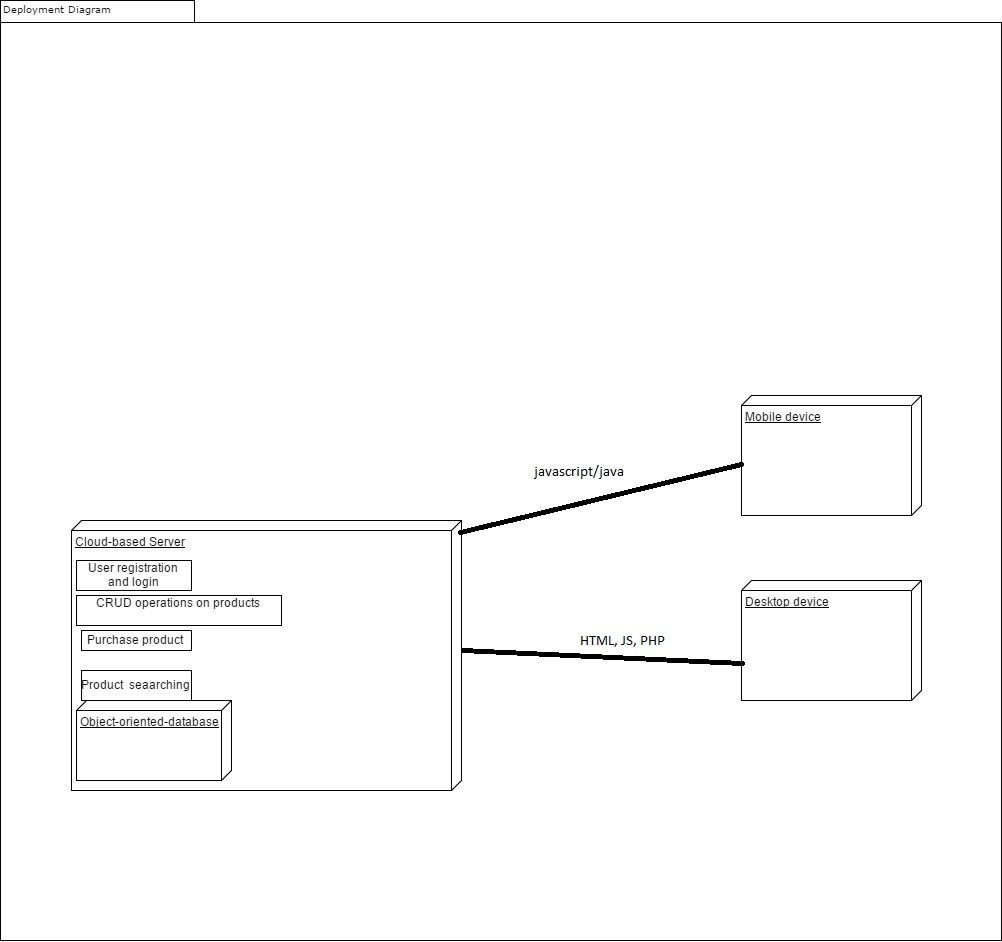
\includegraphics[width=8cm, height=8cm]{Images/purchaseManagementDeploymentDiagram.jpg}\\[1cm]
\end{center}
\subsection{Development Methodology}

e will be utilizing \textbf{Agile} development methodologies with specific reference to \textbf{SCRUM} practices. We believe that this is the best means to enable both us as the engineering team and the client to focus on effectively performing the tasks integral to successfully providing the desired Purchase Management System. 
For this project, Catura will take the part of \emph{Product Owner} and us as Panda Inc will be the \emph{Development Team}. Subsection 3 can be seen as rudimentary version of the \emph{Product Backlog} (which will be further refined/improved in the event of this tender being accepted).
\newline \newline
Interactions are highly valued by our team, hence we are dedicated to conducting weekly or bi-weekly meetings with Retro Rabbit. As stated in the proposal, this will serve and start and end points for \emph{Sprints}. We will also be regularly meeting and consulting with our lectures and tutors for further guidance throughout the duration of the project. All of the above mentioned parties will have access a third party instant messaging platform in order to facilitate communication apart from physical meetings. Our team will be conducting bi-daily \emph{SCRUM meetings} in order to exchange our progress statuses and to ensure an comprehensive mutual understanding is maintained
\newline \newline
A collaborative and cooperative approach between both stakeholders will be employed for the life span of the project. There will also be a focus on the frequent, iterative presentation of small, incremental releases of deliverables to the client. The \textbf{role} of Catura in this approach includes:
\begin{itemize}
\item Active involvement and collaboration in all phases of project
  \begin{itemize}
  \item Analysis and Design - The client will facilitate the identification, definition, prioritisation and continuous refinement of high level requirements, system architecture and design decisions of the Purchase Management Software in order to ensure the correct functionality of the end product.
  \item Development and Deployment - The client will periodically review all instances of the product in order to ensure to it is in line with their expectations 
  \end{itemize}
\item Critical and constructive analysis on not only what we as the engineering team deliver but also on the quality of our service and whether or not we conducted ourselves as would be expected from those in a occupational environment
\item To provide us with the means to produce an effective end product. An exhaustive list of these required means will be provided in further Analysis and Design specification.
  
\end{itemize}
\begin{center}
{\fontfamily{UWR Grotesk}\sffamily\bfseries
\large Thank You Catura. We at Panda Inc. look forward to working with you in the near future.
}
\end{center}
\end{document}
